\section{Actividad No 01 – Valores} 

Los valores introducidos al archivo sysctl.conf ¿que representan?

\begin{itemize}
	\item fssuid dumpable
	\\Los volcados del núcleo pueden contener información que un atacante podría explotar y ocupan una gran cantidad de espacio en disco. Para evitar que el 			sistema cree volcados de memoria cuando el sistema operativo finaliza un programa debido a una violación del segmento u otro error inesperado, se debe 			agregar la siguiente línea al archivo sysctlconf
	\begin{itemize}
			\item VALOR 0  	fssuid dumpable  0
			\\Esto asegurará que los programas de setuid nunca puedan realizar volcados de memoria.
			\item VALOR 1  	fssuid dumpable = 1
			\\Permite volcados de núcleo que pueden ser leídos por el propietario del proceso de dumping.
			\item VALOR 2	 fssuid dumpable = 2	
			\\Permite volcados de núcleo que solo se pueden leer con root fines de depuración.
		\end{itemize}

	\item fsaio max nr
	\\El kernel de Linux proporciona la función de E / S sin bloqueo asíncrono (AIO) que permite que un proceso inicie varias operaciones de E / S 					simultáneamente sin tener que esperar a que se complete ninguna de ellas. Esto ayuda a mejorar el rendimiento de las aplicaciones que pueden solapar el 			procesamiento y la E / S
	\\El rendimiento puede ajustarse utilizando el /proc/sys/fs/aio-max-nrarchivo virtual en el sistema de archivos proc. 
	\\El aio-max-nrparámetro determina el número máximo de solicitudes concurrentes permitidas.
	\\Otro parámetro,, /proc/sys/fs/aio-nrproporciona el número actual de solicitudes asíncronas en todo el sistema.
	\\Se recomienda que establezca el aio-max-nrvalor en 1048576. Esto ayuda a HyperScale a tener un rendimiento óptimo, en un entorno que involucra grandes cargas de trabajo de E / S

\item net.core-rmem.default
	\\El valor por default y maximo de memoria para envio de paquetes.
	\\Un parámetro de kernel que controla el tamaño predeterminado de búferes de recepción utilizado por conectores. Para configurarlo, ejecute el siguiente comando:

\begin{figure}[htb]
\begin{center}
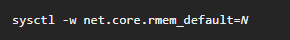
\includegraphics[width=8cm]{./Imagenes/ajhordy}
\end{center}
\end{figure}

Nota:
\\Remplace N por el tamaño en bytes del búfer deseado. Para determinar el valor para este parámetro de kernel, vea {/proc/sys/net/core/rmem\_default} 
\\Tenga en cuenta que el valor de rmem\_default no debería ser mayor que rmem\_max ; en caso de serlo, aumente el valor de rmem\_max.

	\item net.core.rmem.max
	\\Ajusta el m\'aximo de bufer de recepci\'on para todos los protocolos
\vspace*{0.10in}


Nota:
\\Memoria de almacenamiento temporal de informaci\'on que permite transferir los datos entre unidades funcionales con caracter\'isticas de transferencia diferentes.

           \item net.core.wmem.max
\\Por ejemplo, escriba  "sysctl -w net.core.wmem_max = 262144" :
\\Esto establece el tamaño máximo del búfer de envío del sistema operativo para todos los tipos de conexiones.

           \item net.core.wmem_default
\\Por ejemplo, escriba  "sysctl -w net.core.wmem_default = 262144":  
\\Esto establece el tamaño del búfer de envío del sistema operativo predeterminado para todos los tipos de conexiones.

\begin{figure}[htb]
\begin{center}
\\La configuración por defecto en bytes del búfer de envío de socket:
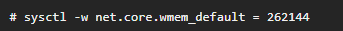
\includegraphics[width=8cm]{./Imagenes/netcorewmendefault}
\end{center}
\end{figure}

Nota: 
\\En resumen dan valor por default y maximo de memoria para envio de paquetes.

\end{itemize} 
